\documentclass[12pt]{article}

\usepackage[margin=1in]{geometry}

\usepackage{amsmath, graphicx, caption, subcaption, xcolor}

\graphicspath{{res/}}

% I need a punchy title which is general enough
% to fit all three (if I can pull them off) points from the lab manual.
\title{\textcolor{red}{The Galactic Plane}}

\author{Lukas Finkbeiner}

\begin{document}

\maketitle

\begin{abstract}

% remember to motivate the paper

We study

1. velocity patterns of various H clouds using Doppler shifts

2. black hole mass

3. accuracy of a spiral arm fit

results, uncertainties.

\end{abstract}

\section{Introduction and Background}
% currently we need more connecting text and MORE MOTIVATION

Given certain patterns, how well does a spiral fit? We need to control for the total number of data. We want the normalization of any two compared sets to be the same (so, we scale accordingly). What numpy functions I used.

\begin{equation} \label{eq:spiral}
R_\text{arm} = R_0 e^{\kappa(\phi - \phi_0)}
\end{equation}

To explore these questions, we want to be able to examine the Doppler velocities and brightness temperatures associated with different parts of the galactic plane of the Milky Way. We want to examine power spectra collected for values of the galactic longitude $\ell$ on the range $-10^\circ$ to $250^\circ$. We will provide a more comprehensive analysis of our particular setup in the methods section. For now, we consider, in the abstract, two equations for calibrating the spectra. 

\begin{equation} \label{eq:line_shape}
T_\text{line} = G \, \frac{s_\text{on}}{s_\text{off}}
\end{equation}

\begin{equation} \label{eq:line_gain}
G = \frac{T_\text{sys, cal} - T_\text{sys, cold}}{\sum{(s_\text{cal} - s_\text{cold})}} \sum{s_\text{cold}}
\end{equation}

The first equation will be used to demonstrate a consistent HI signal by combining spectra for two different frequencies in the local oscillator. The second equation will be used to scale the power spectrum so that the y-axis carries information about the brightness temperatures associated with different frequencies on our spectra.

The following equation is a conclusion of the tangent-point method for converting galactic rotation to Doppler velocity. $R_\odot \approx 220 $ km / s and $R_\odot \approx 8.5$ kpc $\equiv 2.6 \times 10^{17}$ km. 

\begin{equation} \label{eq:vel_dopp}
V_\text{Dopp} = \left[ \frac{V(R)}{R} - \frac{V(R_\odot)}{R_\odot} \right] R_\odot \sin(\ell)
\end{equation}

%\begin{equation}
%\frac{V_\text{Dopp}}{R_\odot \sin \ell} = \frac{V(R)}{R} - \frac{V(R_\odot)}{R_\odot}
%\end{equation}

%\begin{equation}
%\frac{V_\text{Dopp}}{R_\odot \sin \ell} + \frac{V(R_\odot)}{R_\odot} = \frac{V(R)}{R} = \frac{1}{R_\odot} \left[ \frac{V_\text{Dopp}}{\sin \ell} - V(R_\odot) \right] 
%\end{equation}

The following representation will be used in establishing the velocity curve inside the solar circle:

\begin{equation} \label{eq:vel_curve}
V(R) = \frac{R}{R_\odot} \left[ \frac{V_\text{Dopp}}{\sin \ell} - V(R_\odot) \right] 
\end{equation}

%This next form will be used in placing points outside the solar circle, to evaluate the spiral shape:

%\begin{equation}
%\frac{V_\text{Dopp}}{R_\odot \sin \ell} = \frac{V(R)}{R} - \frac{V(R_\odot)}{R_\odot}
%\end{equation}

%\begin{equation}
%\frac{V(R)}{R} = \frac{V_\text{Dopp}}{R_\odot \sin \ell} + \frac{V(R_\odot)}{R_\odot} 
%\end{equation}

%\begin{equation} \label{eq:outer_spiral}
%R = V(R) \left[ \frac{V_\text{Dopp}}{R_\odot \sin \ell} + \frac{V(R_\odot)}{R_\odot} \right]^{-1}
%\end{equation}

In preparation for our mass estimations, we start with the conventional

\begin{equation}
v^2 = \frac{G M_\text{gravitational}}{R} 
\end{equation}

Then, we re-arrange to get the desired form:

\begin{equation} \label{eq:mass}
M_\text{gravitational} = \frac{R v^2}{G} 
\end{equation}

As we collect Doppler velocities for each galactic longitude $\ell$, it is important to distinguish between $\ell$ and the radial distance $R$ of a hydrogen cloud to the galactic center. To estimate mass for the part of the galaxy inside the solar circle, we use the tangent point method by applying equation \ref{eq:vel_curve} with $R = R_\text{min} = R_\odot \sin \ell$. In figure \ref{fig:ell_vs_r}, we illustrate the range of radii associated with an arbitrary $\ell$. The tangent-point method necessarily excludes these other radii. Later on, in the observations section, we will visualize some consequences of this.

\begin{figure}
	\centering
	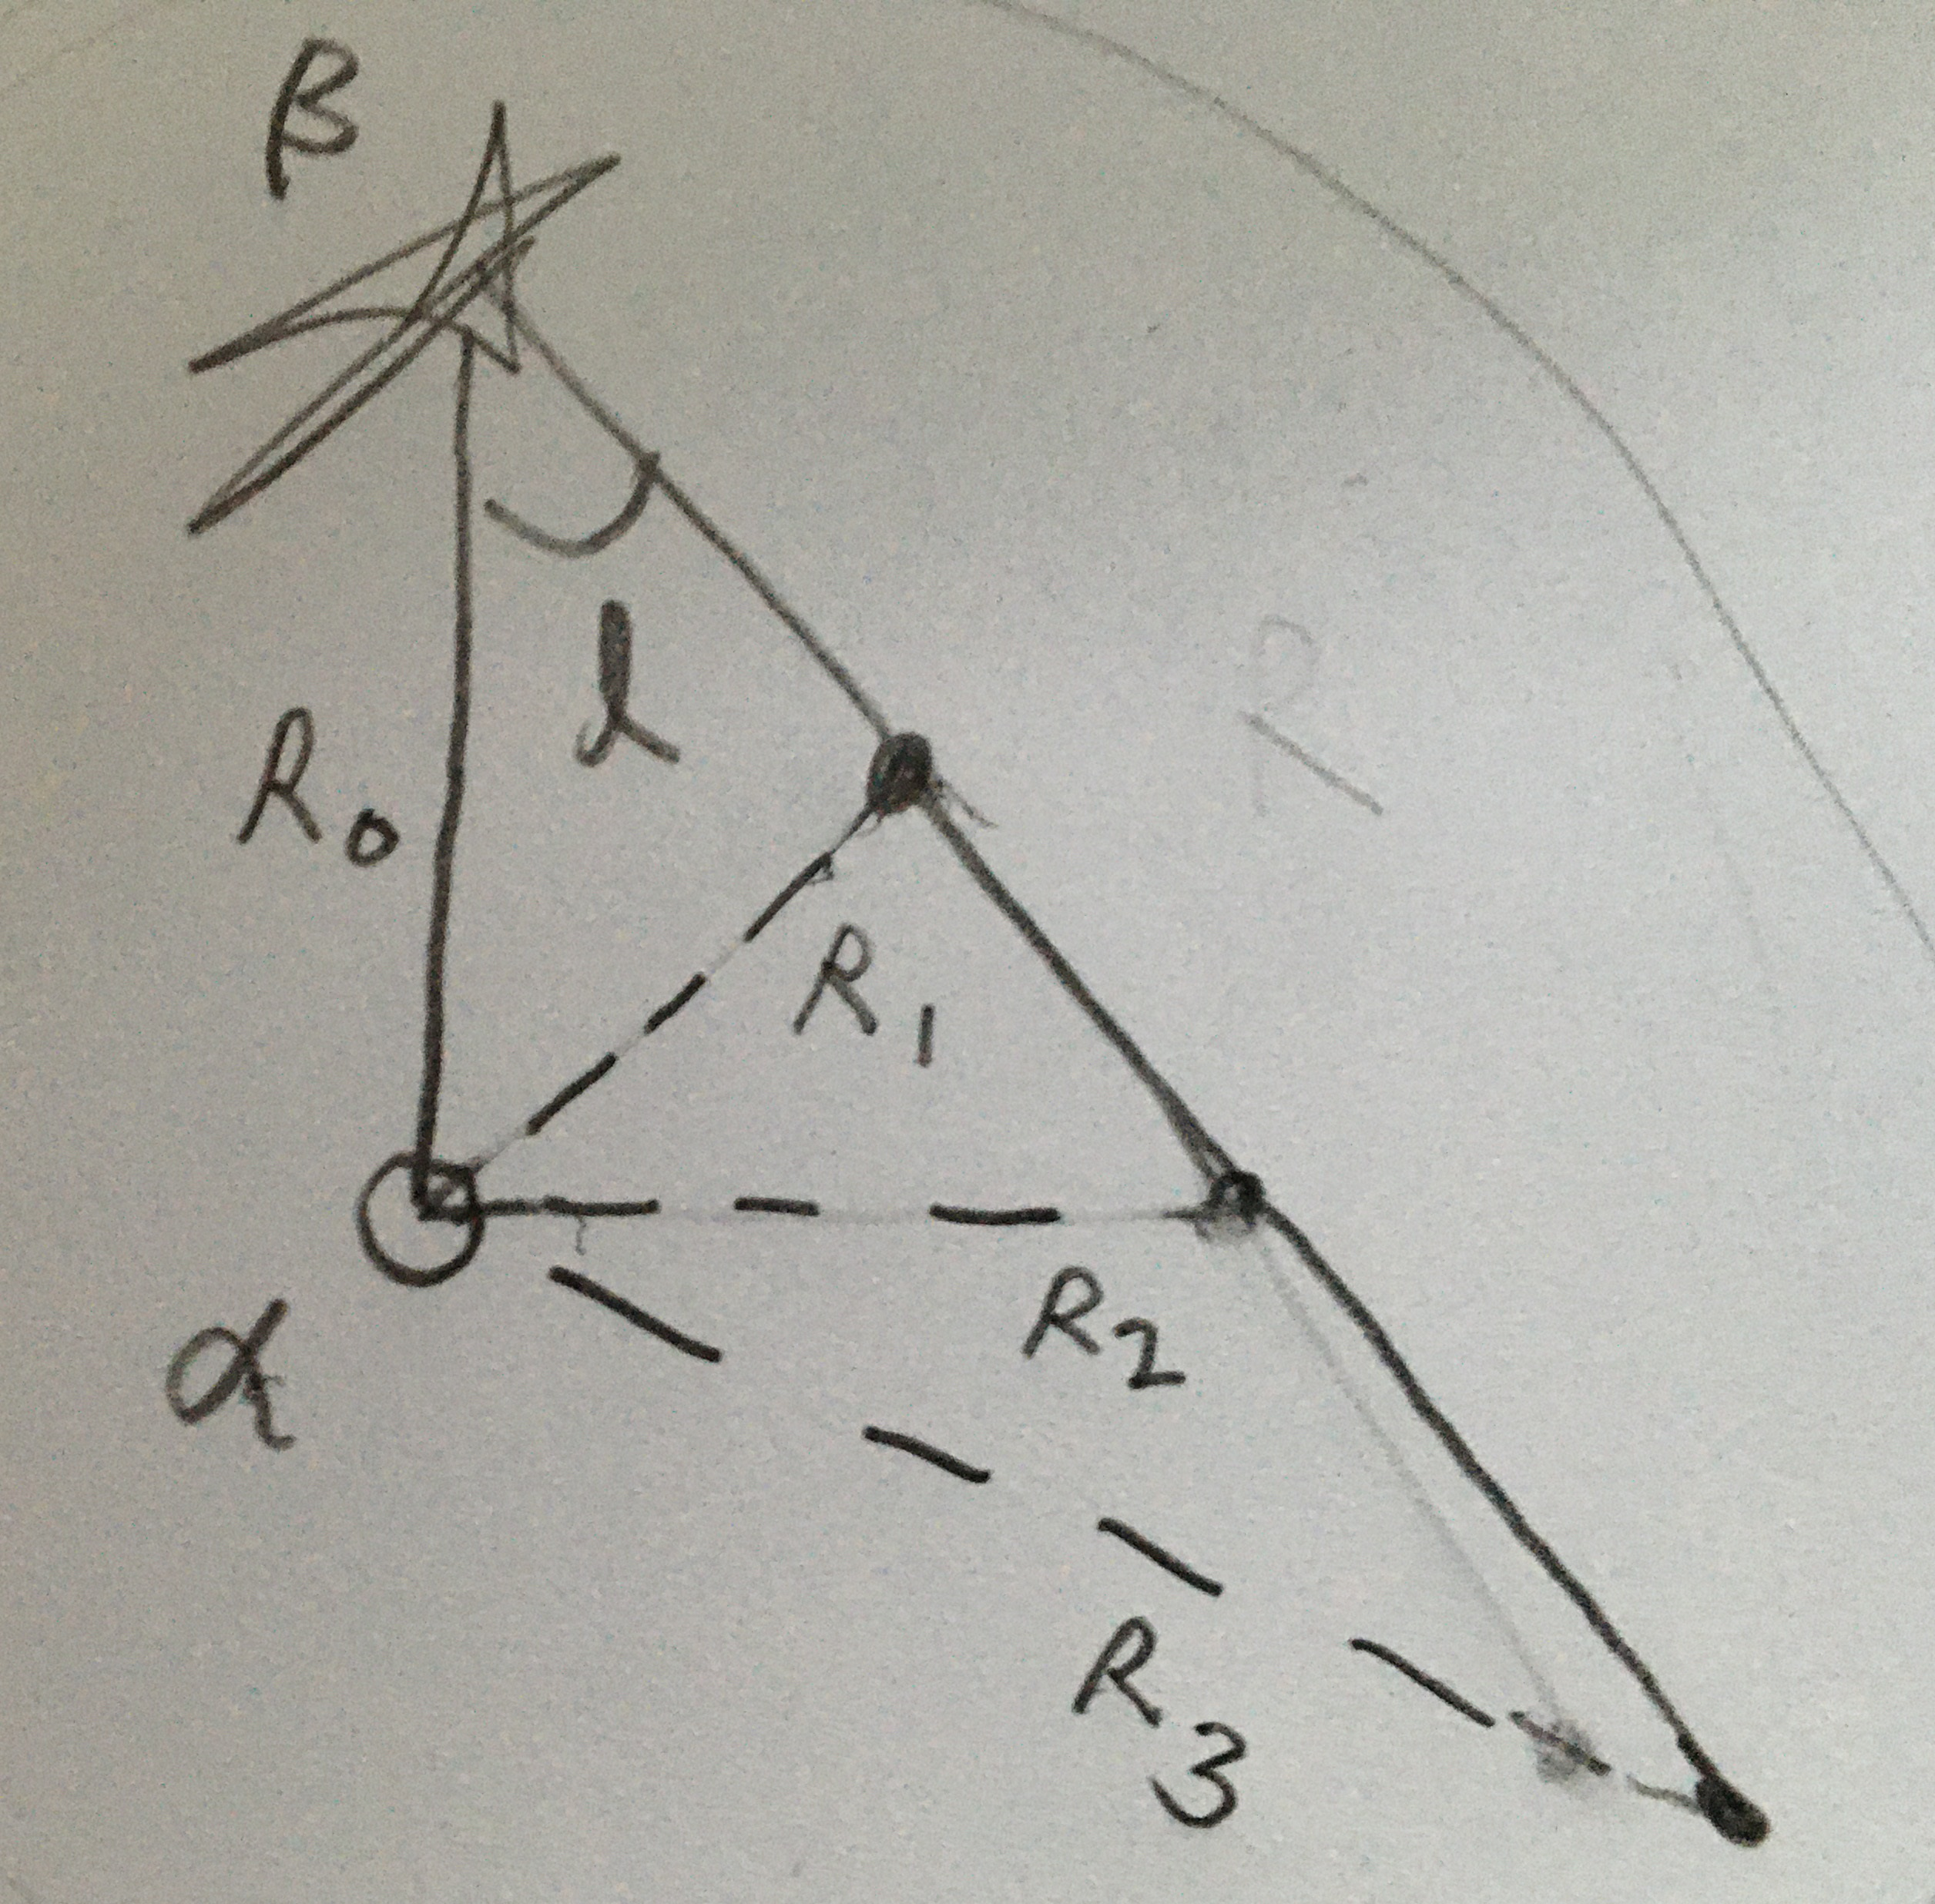
\includegraphics[width=.4\linewidth]{ell_versus_r}
	\caption{This is a simple illustration demonstrating how the value of $\ell$ can place constraints on valid values for $R$ (specifically, $R_2$ here represents the right-triangle case, for which the radius is minimized). However, since our universal value for galactic latitude $b = 0^\circ$ has no relevance to radial distances, no pair of galactic coordinates will specify the radius at which we are working. Consequently, the tangent-point method must explicitly establish that we work with a specific radius $R = R_\text{min}$.}
	\label{fig:ell_vs_r}
\end{figure}

\section{Methods}

\quad \quad To conduct all of our measurements of the galactic plane of the Milky Way, we run a tracking script on a remote computer linked to the Leuschner dish. As a demonstration of the Leuschner dish signal chain (illustrated in figure \ref{fig:sig_chain}), we show how we map a set of input signals to a final frequency axis for our plots (frequency versus brightness temperature). Since we are considering only frequency, this allows us to skip over the amplifiers and attenuators.

\begin{figure}
	\centering
	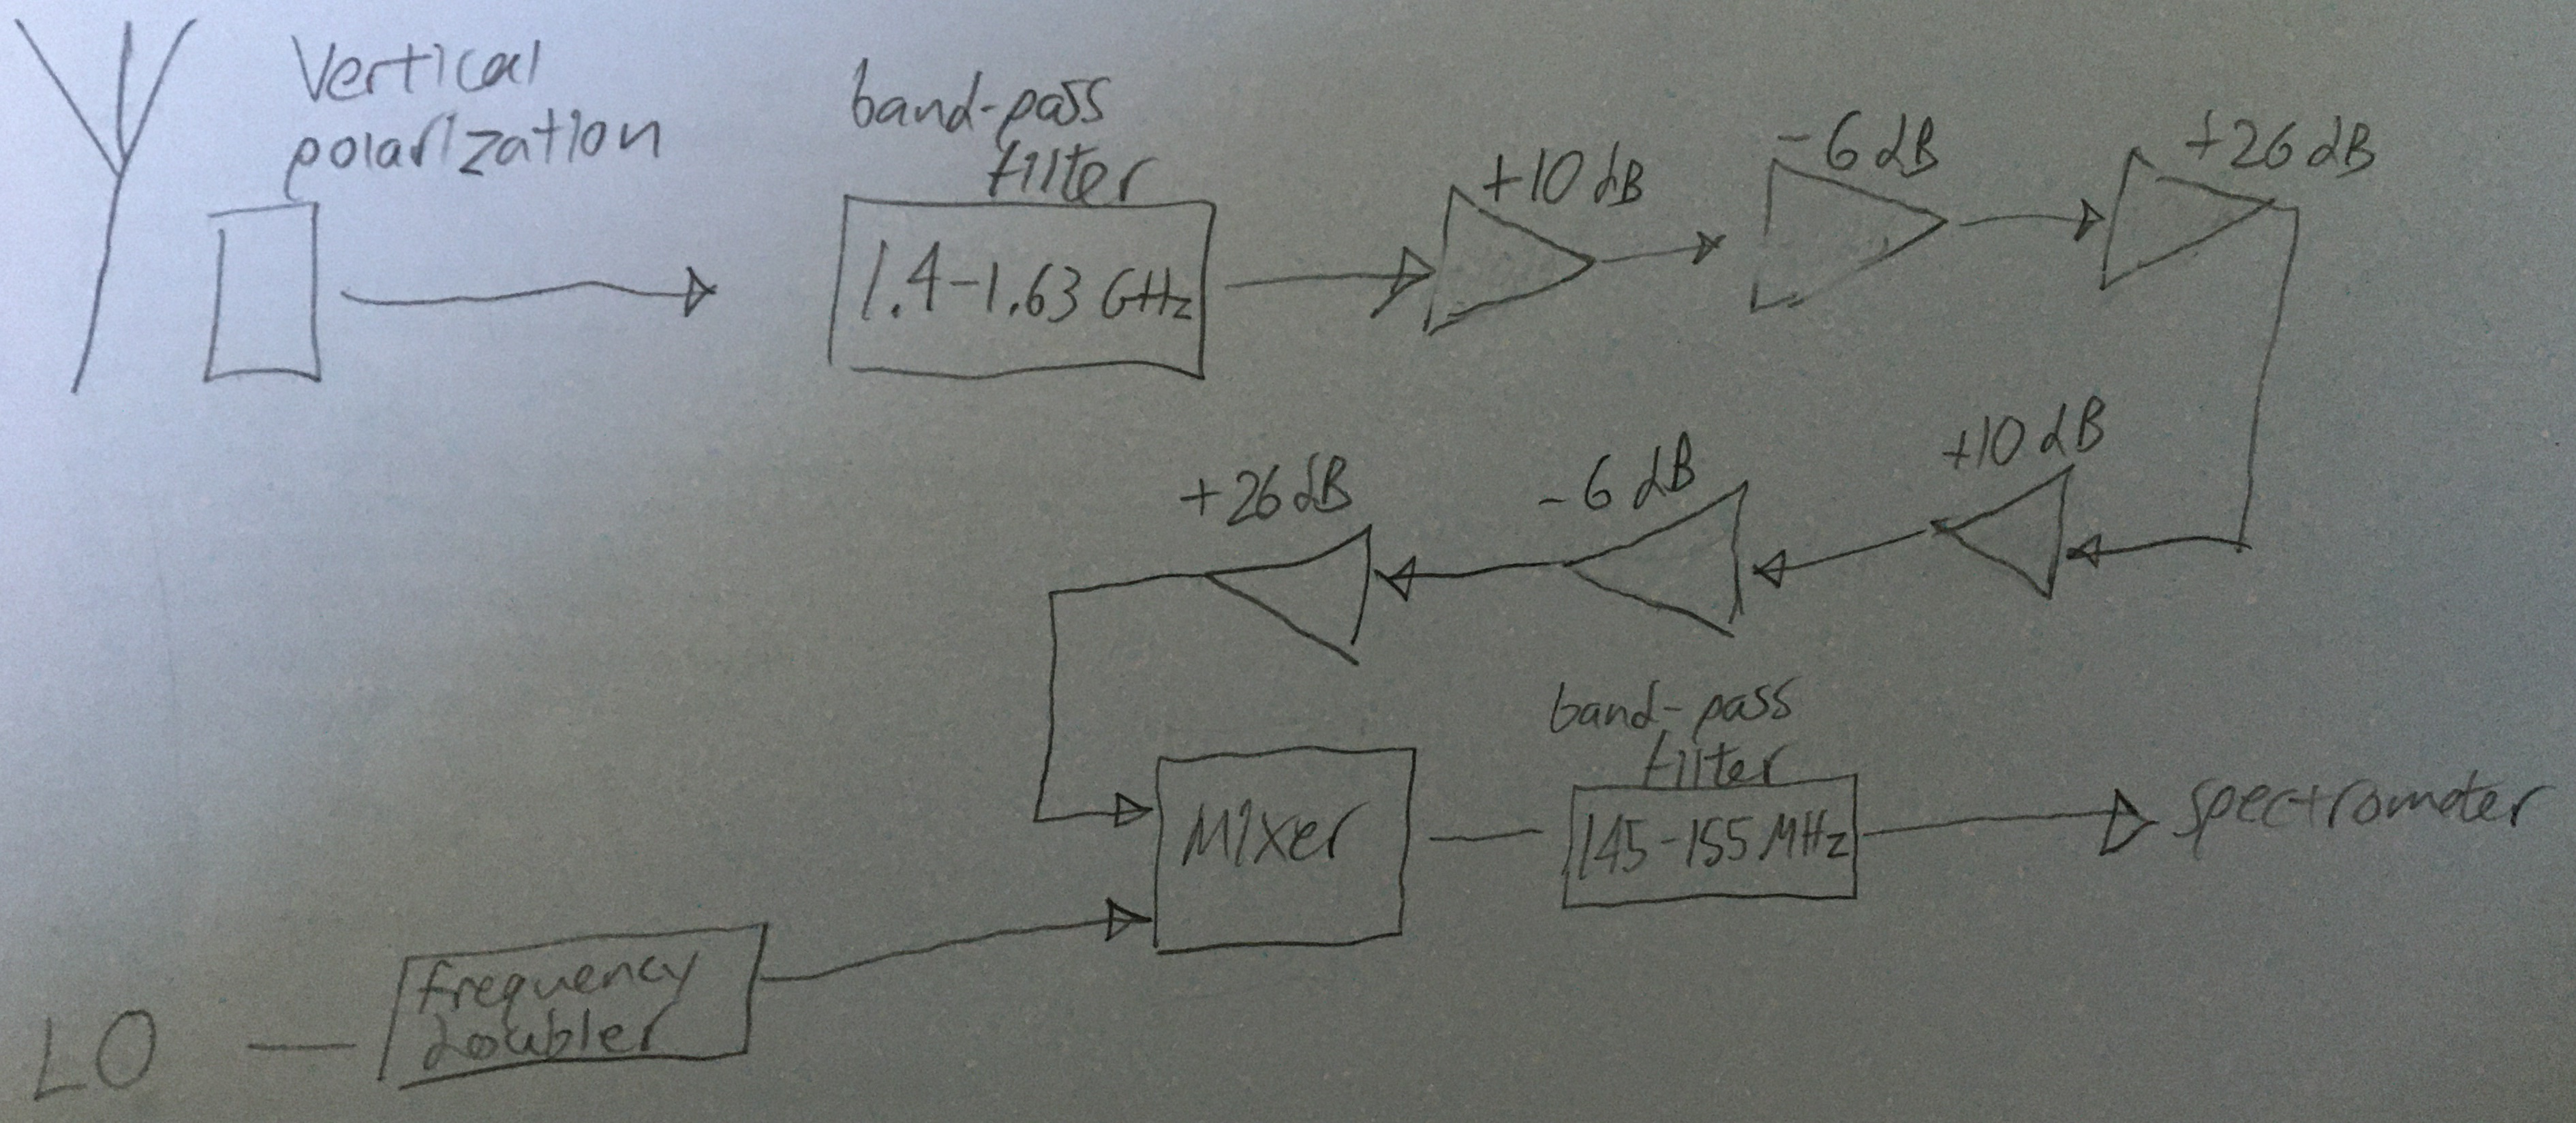
\includegraphics[width=.9\linewidth]{sig_chain}
	\caption{This is a simplification of the Leuschner signal chain, where the horizontal polarization has been ignored (we do not use those data in this report). Furthermore, we abstract-away the clock rate of the ROACH and the various stages of digitization. For our `on' LO frequency of 1270 MHz, the output spectra cover a frequency range 1415 to 1425 MHz.}
	\label{fig:sig_chain}
\end{figure}



The initial band-pass filter ranges from 1.4 to 1.63 GHz. There is a down-converter that mixes this filtered signal with the signal from the local oscillator LO. This leads to a new frequency band (intermediate frequency IF) of 130 MHz to 360 MHz. Since we are using a real-valued mixer, we apply a band-pass filter to eliminate the sum frequencies. This filter is centered at 150 MHz and has a bandwidth of 10 MHz. Consequently, we expect the following frequency range in our outputs (which take the form of spectra in .fits files): a 10 MHz wide range beginning at 145 MHz IF (which maps to 1.415 GHz RF) and ending at 155 MHz IF (which maps to 1.425 GHz RF).

We used 1268 MHz for our second LO frequency, the `off' spectrum. This leads to an output range of 1.417 to 1.419 GHz.

We sample at 24 MHz (we keep 1/32 of the samples from the 768 MHz clock),->12MHz Nyquist bandwidth. so we are operating in the twelfth Nyquist window.

Before we analyze the output of our spectrometer, we need to calibrate the spectra.

We want to change our local oscillator frequency (as shown in figure \ref{fig:sig_chain}) between two values. This allows us to, via the mixer, adjust where the HI line appears in our spectra. We thereby create `on' (LO at 1270 MHz) and `off' (LO at 1268 MHz) spectra.

\ref{eq:line_shape}

The gain, G, is calculated with an additional spectrum ($cal$) that we deliberately contaminate with thermal noise. We do this by activating a noise diode which, for the vertical-polarization receiver (with which we are exclusively concerned here) is independently estimated to contribute about 80 Kelvins. Finally, we compare the magnitudes with a spectrum without this contamination and we compute: \ref{eq:line_gain}



How we calibrate: for each value $\ell$, we take four sets of ten spectra: ...

We convert from galactic to topocentric coordinates using rotation matrices, as described in a previous report. How much should I include? If I describe the matrices again, that will certainly have to go in the introduction.

We probably want a basic run-down of a .fits file, but perhaps some of that can go in the introduction.

\begin{figure}
	\centering
	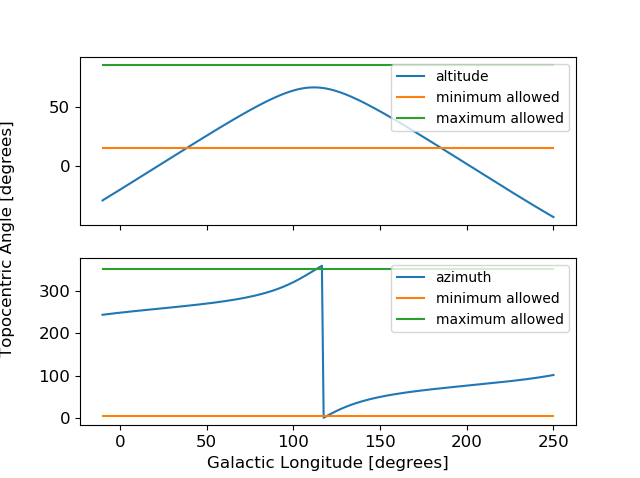
\includegraphics[width=.75\linewidth]{1940_10_05_2020}
	\caption{This is a visibility demonstration to clarify our observation process: we input a value for the local sidereal time, and our script plots the topocentric coordinate conversions for all values of the galactic longitude $\ell$ on our range (since we are observing the galactic plane, the galactic latitude $b$ is universally zero degrees). We began this project with the nominal range of $\ell \in [-10^\circ, 250^\circ]$. By calculating similar visibility curves for a full sidereal day, we are able to classify some of our observations with higher risk for obstruction (particularly when the target altitude is close to the dish's minimum attainable altitude).}
	\label{fig:vis_demo}
\end{figure}

\section{Observations}

\quad \quad What would be a good $introduction$ to the data? We have hundreds of raw spectra. I am not sure how to $succinctly$ describe observations before we get into the analysis.

\begin{figure}
	\centering
	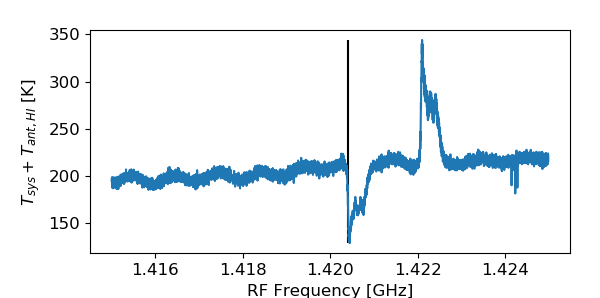
\includegraphics[width=.8\linewidth]{cal_ex_80_deg}
	\caption{Here is an example of a fully calibrated example ($\ell = 80^\circ$), just one of 260. There is a black vertical line indicating the location of the 21 cm HI line at rest (1420.405751786 MHz at rest).}
	\label{fig:cal_ex}
\end{figure}

% This plot is simply a way of concisely representing the 260 spectra we collected over the interval $\ell \in [-9, 250]$ degrees (one-degree spacings).
\begin{figure}
	\centering
	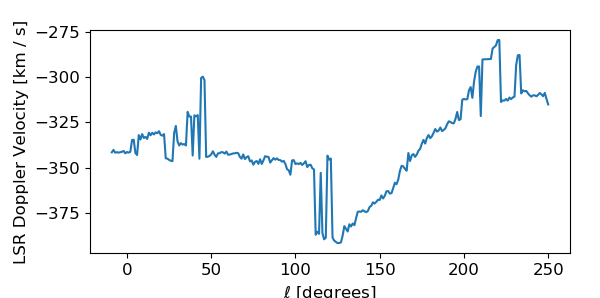
\includegraphics[width=.8\linewidth]{Doppler_collection}
	\caption{We take the peak intensity of each spectrum to represent the shifted HI line for that galactic longitude.  Observe that, for our tangent-point considerations ($\ell \in [0, 90]$), we have an initial region featuring wild fluctuations followed by a relatively flat region for the second half of the angles. While this could represent physical realities, this seeming discontinuity of the derivative could also be a consequence of the primitive intensity-maximizing function, or it could be a consequence of pointing the telescope at angles close to mechanical boundaries. \textcolor{red}{This is $almost$ the image $T_A(\ell, V_\text{LSR})$; we need the brightness temperature associated with each Doppler velocity, then we can color this.}}
	\label{fig:Dopp_collection}
\end{figure}

\begin{figure}
	\centering
	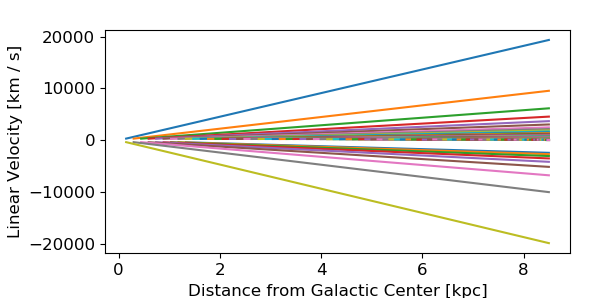
\includegraphics[width=.8\linewidth]{tangentPoint_dispersion}
	\caption{This is an overplot of all 90 possible velocity curves. Specifically, when we treat the solar circle of the galaxy, we know that for each $\ell$, $R$ can take on a maximum value of $R_\odot$ (the radius of the solar circle) and a minimum value of $R_\odot \sin \ell$. The tangent-point method mandates the usage of $R_\text{min}$, but we here demonstrate how that method necessitates the collapse of line segments into points.}
	\label{fig:TP_disp}
\end{figure}

\begin{figure}
	\centering
	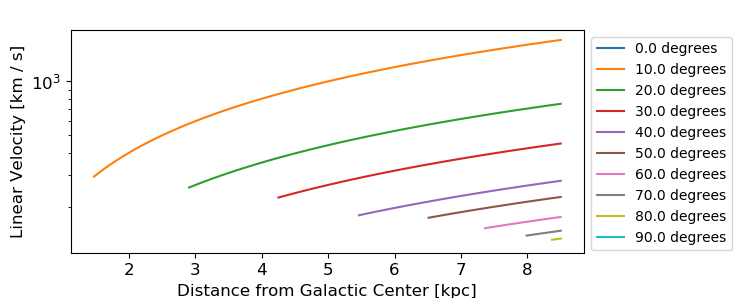
\includegraphics[width=.9\linewidth]{tangentPoint_selected_dispersions}
	\caption{Here we are essentially representing similar information to that of figure \ref{fig:TP_disp}. We use a semilog vertical axis to verify that there is one consistently-varying multiplicative offset ($\frac{1}{\sin \ell}$) as we examine different galactic longitudes. This plot also agrees with our expectation that our two boundary cases are meaningless: $\ell = 0^\circ$ approaches an infinite linear velocity and $\ell = 90^\circ$ corresponds to a velocity curve for which the minimum and maximum radii are the same (an infinitesimal segment).}
	\label{fig:TP_sel_disp}
\end{figure}

\section{Analysis}

\quad \quad We can estimate the mass of the whole galaxy like this. We can estimate the mass within the solar circle like this. What fraction is gas, and what fraction is star? Does this question not require a given nuber for the mass of all stars?

We can estimate the mass of the super-massive black hole at the center of the milky way if we use the Doppler velocity for our closest angle ($\ell = 1^\circ$) and combine equations \ref{eq:vel_curve} and \ref{eq:mass} and integrate over radii from the galactic center out to a single light-year. According to \textcolor{red}{blah}, the active galactic nucleus is about $4.4 \times 10^{7}$ km in radius. By comparison, a light year is six orders of magnitude larger than the estimated radius of the black hole. \textcolor{red}{I have no idea what is going on.}

The result? Mass $\approx 7.6405 \times 10^{13}$ kg. This is seventeen orders of magnitude below the mass of the sun. Something has gone terribly wrong. Even if I were to expand to expand my range of radii to 10000 times the radius of the black hole, I would still be at three-quarters the mass of our sun. 

\begin{figure}
	\centering
	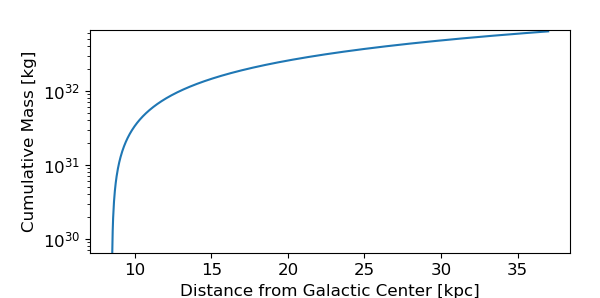
\includegraphics[width=.8\linewidth]{outer_mass_distro}
	\caption{This is a cumulative mass distribution for radii larger than that of the solar circle. The plot begins with a mass of zero because we subtract-off whatever the function calculates for radii smaller than that of the solar circle; we know the calculations to be erroneous for the smaller radii because we are applying different calculation methods. Observe that the rate of increase of mass drops off rather steeply. We hope for this to be the case as the galaxy thins out toward its edges and is most dense at smaller radii.}
	\label{fig:outer_mass_distro}
\end{figure}

\begin{figure}
	\centering
	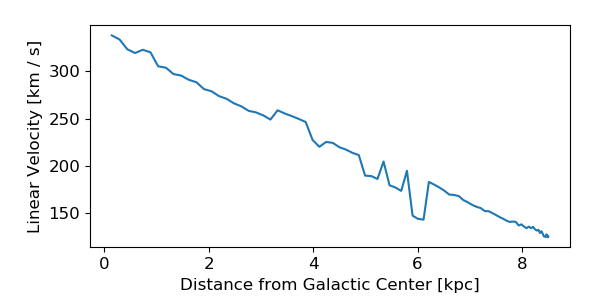
\includegraphics[width=.8\linewidth]{inner_vel_distro}
	\caption{This is a plot of galactic rotation velocities by radius, calculated using the tangent-point method. If we approximated the galactic plane as a rigid disk, we would expect the velocity to increase with greater radius (as the same angular distance must be covered in the same amount of time at a greater radius). While this line does not disqualify a spiral, we might initially expect a spiral shape to come from $similar$ linear velocities manifesting as curved arms at greater radii. It is not clear if the fall-off of gravitational influence would agree with this model.}
	\label{fig:inner_vel_distro}
\end{figure}

\begin{figure}
	\centering
	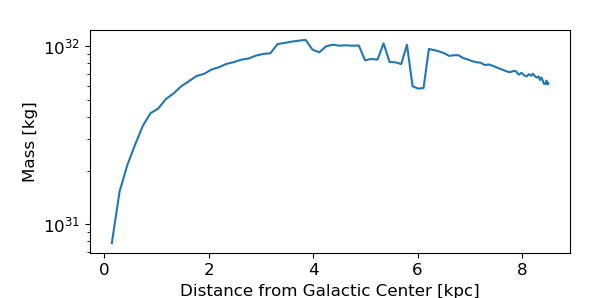
\includegraphics[width=.8\linewidth]{inner_mass_distro}
	\caption{This is a semilog plot of interstellar cloud mass versus radius. The calculation rests conceptually on a cumulative distribution function, so we may immediately spot imperfections in the data. Specifically, after about 3 kpc, the data do not leveling off consistently. Instead, the mass response fluctuates and then slowly declines. However, the initial rise does fit with our expectation of a general decrease in density as we move outward from the center.}
	\label{fig:inner_mass_distro}
\end{figure}

\section{Conclusions}

\quad \quad We seem to have at least a couple of results! How do I estimate the uncertainty on the Leuschner dish?

\section{Acknowledgments}

\quad \quad Who did what?

Theory and background provided by Aaron Parsons. ``LAB 4: Mapping the Galactic HI Line.'' Updated April 2020.

% Can we please get a bibliography this time?

% The following is a lorem ipsum. We want
	% tangent-point resource recommended by Rebecca
	% my source for the radius of the galactic black hole
	% lab 2, for most of the gain and line shape stuff. Should I also cite myself?

\begin{thebibliography}{9}
\bibitem{latexcompanion} 
Michel Goossens, Frank Mittelbach, and Alexander Samarin. 
\textit{The \LaTeX\ Companion}. 
Addison-Wesley, Reading, Massachusetts, 1993.

\bibitem{einstein} 
Albert Einstein. 
\textit{Zur Elektrodynamik bewegter K{\"o}rper}. (German) 
[\textit{On the electrodynamics of moving bodies}]. 
Annalen der Physik, 322(10):891–921, 1905.

\bibitem{knuthwebsite} 
Knuth: Computers and Typesetting,
\\\texttt{http://www-cs-faculty.stanford.edu/\~{}uno/abcde.html}
\end{thebibliography}

\end{document}
